\chapter{Introduction}
\label{chapter:introduction}

In the past few years, \gls{AI} has experienced an unprecedented growth in both industry and research.
This was made possible by advances in \gls{ML} and statistics but also thanks to the computing capacities of modern \gls{GPU}.
A broad spectrum of domains enjoys the fallouts: medicine, law, digital marketing, finance, automobile industry, and so on.
The overwhelming majority of applications involves predicting outcome given an input in a stateless fashion.
For example, using image recognition, a radiologist may get help finding tumours on an x-ray image; given a sentence, an automatic translation tool infers the same sentence in an other language; a trading black-box predicts the next variation of a stock with the knowledge of all the past variations in stock exchange.
When the task involves interacting with the \idx{environment} in a sequential fashion, the tools used to solve all the aforementioned problems do not suffice. This class of problems includes - among others - autonomous driving, power-grid management, online advertising, video games, robotics, and the domain this work focuses on: dialogue.


%In \acrlongpl{DS},
In dialogue applications, two \idx{agent}s interact with each others.
A classic use-case is an \idx{agent}, called \gls{DS}, interacting with a human user.
To that end, one must designs the strategy the \gls{DS} will adopt. While pioneer methods involve rule-based \glspl{DS}, recent solutions involve learning the \gls{DS} strategy, or \textit{\idx{policy}}, using the \gls{RL} framework.
The basic idea is that an \textit{\idx{agent}} (the \gls{DS}) interacts with the \textit{\idx{environment}} (the user).
As it is interacting, the \idx{agent} \textit{reinforces} its knowledge of the \idx{environment} and adapts its \idx{policy} accordingly.
One drawback of this method is it may need a substantial amount of interactions to construct a good enough \idx{policy}.
This statement is especially true during early interactions. Correspondingly, if a human tries to solve a completely new task, for instance, operating weightlessness with a full spacesuit, he will fail or, at the very best, face some issues in his first interactions, then eventually adapt to the new \idx{environment}. Because space missions are expensive and time is critical, and for probably a lot of additional factors out of the scope of this thesis, an astronaut cannot afford to learn from scratch this new task.
%!TU: dommage, ce serait cool de prevoir un voyage spacial en these :)
%
To remedy this situation, astronauts are trained to execute a set of tasks equipped with their suit, in a weightless pool on Earth. That way, they will be able to \textit{\idx{transfer}} their knowledge gathered in the pool \idx{environment} to quickly adapt in the space \idx{environment}. Now, we consider that the astronaut represents the \gls{DS}, the pool \idx{environment} represents a young person used to new technologies and the space \idx{environment} represents an elderly person with a very weak control over new technologies. If one trains a \gls{DS} enough to interact flawlessly with the young person, then he may be able to \idx{transfer} the data, the \idx{model} or even the learnt world representation (\textit{features}\index{feature}) to a new \gls{DS}, in order to speed-up the learning when interacting with the elderly person. In \gls{ML}, this process is called \gls{TL} and this thesis makes the hypothesis that \gls{TL} should be a good fit to improve the learning of \glspl{DS}.


\section{History of dialogue systems}

In the collective imagination, a robot should walk, execute tasks, interact, and seamlessly talk with humans. Each of these abilities is actually a whole domain of research. For now, the separation is clear between each domain\footnote{Even if one could argue that everything is connected, as for example, it may be hard to converse with a robot that is running around.}. Science fiction introduced intelligent \idx{agent}s that can dialogue; while Hal9000~\parencite{hal9000} or Kit~\parencite{k2000} talk and control a fully mechanical body (a spaceship and a car respectively), the sole purpose of the Multivac~\parencite{multivac} is question answering. In the same fashion, this thesis focuses on building intelligent agents\index{agent}, known as \glspl{DS}, where the sole purpose is to interact with the human through the voice and using text. To build a \gls{DS}, the designer must solve the following challenges: process the human voice, extract meanings, decide what to respond, create a proper \idx{semantic} for the response and, finally, generate the artificial speech signal for the response. While this thesis focuses on the decision part (also called \gls{DM}), a lot of research has been conducted on the other domains, independently from \gls{DS} in a whole.


\paragraph{Processing and generating speech}

While text-based \glspl{DS} process text information and produce textual answers, \gls{SDS} interact with the users through the voice channel. The challenging task for \glspl{SDS} is then to understand and generate spoken sentences (text to audio and audio to text). Solutions incrementally more and more impressive trough the years have been proposed from the signal processing community in the 20th century. For these particular tasks, two modules are involved and detailed in \Cref{chapter:the-pipeline}, the \gls{ASR} module used to process user spoken language, and the \gls{TTS} module to produce the system spoken response.

% the natural language understanding module (NLU) to extract meaning from the

\begin{wrapfigure}{R}{0.5\textwidth}
    \centering
    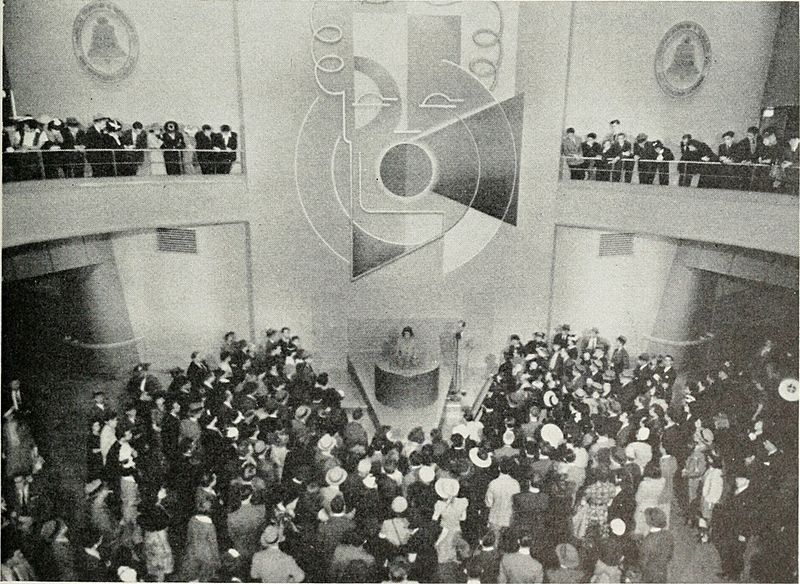
\includegraphics[width=0.5\textwidth]{sources/introduction/voder-fair.jpg}
    \caption{\label{fig:world-fair} The Voder demonstration}
    %\addcontentsline{toc}{figure}{Figure \Cref{fig:world-fair}} % Uncomment to add the figure to the table of contents
\end{wrapfigure}

The first solution to the speech synthesis problem, known as \gls{TTS}, was the Voice Operating Demonstrator known as Voder~\parencite{voder}. It is an electronic machine able to synthesise human speech using a dedicated keyboard. It is based on Dudley's work at Bell Lab on the vocoder, a tool to analyse and synthesise speech. The Voder has been introduced at the 1939 New York World's Fair as show in \Cref{fig:world-fair}. In 1950, Dr. Franklin S. Cooper from Haskins Laboratories released the final version of the Pattern playback~\parencite{pattern-plaback}. This device generates sounds given spectrograms of speech patterns. In the end of the 20th century, the dominating speech synthesizer was DECtalk. The system is based on early work on KlattTalk~\parencite{klatttalk}. The system itself was a standalone pluggable on any telephone facilitating vocal servers. Recently, DeepMind showed impressive results with WaveNet~\parencite{wavenet}, a deep \gls{NN} for generating raw audio waveforms. The network is able to generate speech in many languages but also novel music fragments. The same company introduced very recently a \gls{GAN} approach for \gls{TTS} \parencite{bikowski2019high}.

The earliest attempt at designing an \gls{ASR} module was successfully achieved by the Elmwood Button Company with Radio Rex. It was a toy dog built to react to simple sound patterns, like "Rex". In the late 1940s, the military got involved, when the U.S. Department of Defense sponsored the first researches in \idx{speech recognition} in order to process automatically intercepted Russian messages. Following up, numerous systems were able to processing digits~\parencite{davis1952automatic}, vowels~\parencite{forgie} and finally words~\parencite{gold}.
It is in the 1970's that the Defense Advanced Research Projects Agency (from the U.S. Department of Defense) ran a massive \idx{speech recognition} program involving well-established research groups, this attempt was unsuccessful but it led to a new area of research around \glspl{HMM}~\parencite{hmm}.
\glspl{HMM} were a first step in the art of learning statistical models\index{model} based on data. \glspl{HMM} were a reference in \gls{ASR} until the perceptron~\parencite{Rosenblatt58theperceptron} expanded into \glspl{NN}. \gls{HMM} approaches involve different modules to handle pronunciation, acoustics and language \idx{model}. \glspl{NN} shift the problem to an end to end approach, i.e. sound signal to sentence. To that extent, \gls{RNN}~\parencite{rnn}, and later \gls{LSTM}~\parencite{lstm}, have been applied to predict sequences of words~\parencite{rnn-asr}.

\paragraph{On the semantic problematic}

Two components of a \gls{DS}, the \gls{NLG} and the \gls{NLU} handle most of the \idx{semantic}s involved in the \idx{dialogue} process. The \gls{NLU} transforms text to concepts/\idx{semantic}s, the \gls{NLG} does the opposite.

Research in \glspl{NLG} started growing in 1970. Several applications benefited from the advances as text summary~\parencite{nlg-weather-forecast} and documentation generation~\parencite{poo-nlg}. The \glspl{SDS} have been using template-based \gls{NLG} for a long time. The first fully automated \gls{NLG} for \glspl{SDS} were developed in the early 2000s~\parencite{oh2000stochastic,rambow}. In ~\textcite{lemon2011learning}, the \gls{NLG} module from the \gls{SDS} and the \gls{DM} (as discussed in ~\Cref{chapter:the-pipeline}) are jointly optimised. Later,~\textcite{survey-nlg} survey described 12 years of advances in \glspl{NLG} research. More recently, \glspl{NN} have been used to automatically generate behavior explanations of an autonomous \idx{agent}~\parencite{Ehsan:2018:RNM:3278721.3278736}.

Meanwhile, in the same period, research around \gls{NLU} has been conducted. In 1954, the Georgetown–IBM experiment has been conducted in order to process automatic translations of Russian sentences to English using grammar rules. Then, during his Ph.D thesis, Daniel Bobrow developped STUDENT, a program solving algebra word problems~\parencite{nlu-bobrow}. In 1969, Roger Schank introduced the conceptual dependency theory~\parencite{nlu-concept}: the idea was to share the same representation for two sentences with equivalent meaning. Later, \gls{ML} methods have been used for \gls{NLU} with, for example, statistical pattern-matching ~\parencite{Allen:1995:NLU:199291}. The next millennium saw IBM Watson, supercomputer champion of the Jeopardy?!, using the deepQA technology~\parencite{Ferrucci2010}. Finally, more recent approaches use \glspl{NN}.


\paragraph{The Turing-Test}

The ground basis of \glspl{DS}, and computer science in general, has been established by Alan \idx{Turing}. He was a mathematician and logician and he is notably known as the first computer scientist in the modern term's meaning. His well known contributions are the \idx{Turing-Machine}~\parencite{turing-maching} and the \idx{Turing-Test}~\parencite{turing-test} both in scientific world and popular culture\footnote{To name a few: in the movie Blade Runner~\parencite{blade-runner}, the Voight-Kampff test is a \idx{Turing}-like test to identify replicants (robots). More recently, the whole plot of Ex-machina~\parencite{ex-machina} is around the \idx{Turing-Test}. In the Imitation Game~\parencite{imitation-game}, we learn how Alan \idx{Turing} and his team deciphered the Enigma German machine using a dedicated electro-mechanical device (called the
\idx{Turing-bombe}), potentially shortening World War II of a few years.}.

Quote~\ref{quote:bliss} gives a rough idea of what is the \idx{Turing-Test}. This test is inspired by the imitation game, where an interrogator must determinate the gender of a human, based only on written interrogations. While the imitation game discriminates males from females, the \idx{Turing-Test} discriminates humans from machines. This test is designed to measure the human-likelihood of a \gls{DS}. A human, the tester, dialogues\index{dialogue} independently with two agents\index{agent} hidden in a box. One \idx{agent} is another human, the other is the \gls{DS}. If the tester is unable to tell which is the human and which is the artificial system, then the test is successful.


\begin{quote}{\selectlanguage{english}
\begin{description}[noitemsep = 0pt]%style = nextline,
    \item[Bliss:]  Isn't it possible I may be so cleverly artificial that in every respect, from largest to smallest, I am indistinguishable from the natural. If I were, how could you tell the difference between me and a true human being? ? $[\dots]$

    \item[Janov:] It seems to me, then, that a robot that can in no way be distinguished from a human being is a human being. If you were such a robot, you would be nothing but a human being to me.

\end{description}}
    \captionof{floatquote}{
    A \idx{dialogue} between Bliss and Janov Perolat about discriminating Bliss as a robot or not, in Foundation and Earth \parencite{asimov-foundationandearth}
    }
    \label{quote:bliss}
\end{quote}

Recent attemps in the \idx{dialogue} community proposed automatic almost-\idx{Turing-Test} or scores. The BLEU score~\parencite{BLEU}  was introduced to measure the human-likeness of an automatic translation. The ROUGE score~\parencite{ROUGE} evaluates the quality of an automatic text summary. ADEM~\parencite{ADEM} is an automatic \idx{dialogue} evaluator learnt on datasets of human evaluations.

\paragraph{Dialogue Systems}

Previously covered technologies were not \glspl{DS} strictly speaking but rather individual technologies later used as components of \glspl{DS}. The first actual textual \gls{DS} which
 was capable of attempting the \idx{Turing-Test} is ELIZA~\parencite{ELIZA}. It is a text-based \gls{DS} (chatbot) used to mimic a Rogerian psychotherapist~\parencite{rogerian}; it reformulates vaguely what the patient said in order to express empathy. In 1972, the psychiatrist Kenneth Colby created PARRY~\parencite{parry}, a textual \gls{DS} simulating a person with paranoid schizophrenia. This program also passed the \idx{Turing-Test} when psychiatrists were unable to discriminate PARRY from a human patient better than random guessing. In 1972, three major technologies of the 70s met; during the International Conference on Computer Communication, PARRY and ELIZA exchanged through the ARPANET, the ancestor of the Internet. We can already distinguish two types of \glspl{DS}, a chatbot, ELIZA, and an \idx{user-model}, PARRY, which simulates a real human user. In 1977, Daniel Bobrow introduced the Genial Understander System as one of the first \idx{task-oriented} \gls{DS} in the form of a travel \idx{agent}~\parencite{gus}. In 1995, the Massachusset Institute of Technology released Voyager~\parencite{voyager}, an \gls{SDS} for urban navigation. It was quickly followed by Jupiter, from the same laboratory, a telephonic \gls{SDS} for weather information~\parencite{jupiter}. Meanwhile, Orange created ARTIMIS~\parencite{sadek1997artimis}, a \gls{DS} based on the idea of rational agency, where the dialogue can be seen as rational interactions using logical axioms~\parencite{cummings2010routledge}. In 1996, the company Charles Schwab released the eSchwab, an internet service for stock information~\parencite{cortada2005digital}. They designed the service as a \gls{DS} using all the aforementioned modules (\gls{ASR}, \gls{NLU} etc)~\parencite{these-pietquin}.

Marilyn Walker was the first to cast the \gls{DS}'s strategy as a stochastic optimization problem~\parencite{walker1993informational}, followed closely by  \textcite{biermann1996composition}, and later by ~\textcite{walker1998learning}, with real users experiments. Meanwhile, Esther Levin was the first to formally describe \idx{dialogue} management as a \gls{MDP} problem~\parencite{first-mdp-sds}. Then \glspl{POMDP} ~\parencite{pomdp} have been extensively used for \idx{dialogue} management~\parencite{roy2000spoken,pomdp-sds}. The \gls{DM} uses belief tracking (or \gls{DST}), i.e. summary of the current state of the \idx{dialogue} using \idx{dialogue} history. It led to the \gls{DSTC} ~\parencite{dstc}, a competition evaluating the best \idx{model}s for belief tracking. \glspl{RNN} did very well at this task~\parencite{dstc-rnn}.

\section{A challenge for modern applications}

\acrlongpl{DS} are autonomous agents\index{agent} intended to converse with humans (or even another \gls{DS}). The state-of-the-art algorithms are now data-driven solutions~\parencite{lemon2012data}; this ability to automatically process voice or text from a user can improve considerably any application based on a human-machine interface. In the movie Her~\parencite{her}, the dialoguing entity, an overpowered vocal assistant pretty close to Artificial General Intelligence, can process or deliver any kind of information and comes along with a lot a features\index{feature} that cover anything a human could offer and more. In real life, for now, \idx{dialogue} applications are divided in three parts, corresponding to three kinds of problems~\parencite{Gao2018-neural-approches-convertional-ai}:

\paragraph{Social chat} The \glspl{DS} converses with the user like it would do passing the \idx{Turing-Test}. The conversation is mainly chit-chat with some recommendations and there is no well-defined goal. The purpose of these systems is entertainment-driven. To that end, systems are mainly trained to reproduce human conversation using predictive models\index{model} or retrieval-based methods~\parencite{chen2017-survey-sds}. Mitsuku~\parencite{mitsuku} and Rose~\parencite{rose} are examples of chit-chat applications available on the market. Chit-chat can be also involved in the other \idx{dialogue} problems; in the online shopping domain, while the \gls{DS} actually performs a task, 80\% of the utterances are chit-chat messages~\parencite{Yan2017-sds-online-shopping}.


\paragraph{Question answering} In a more pragmatic way, the \gls{DS} must provide a direct and concise answer to user queries containing all the information needed. Most of the research focuses solely on query question answering. So the system extracts keywords from the user query with \idx{semantic} parsing then consults a database (web documents or knowledge bases such as sales and marketing datasets) to get the information.
It reformulates this information with natural language paraphrasing in a human way. State-of-the-art vocal assistants (Google assistant, Amazon Alexa, etc) solve this kind of problems~\parencite{mobile-speech-solution}. Recently, OpenAI team introduced GPT-2~\parencite{radford2019language}, a Transformer architecture~\parencite{vaswani2017attention} that is able to do extremly realistic question answering and text-autocompletion.


\paragraph{Task completion} The \gls{DS} must achieve a task based on the information provided by the user. It usually takes multiple \idx{dialogue} turns\index{turn} to gather all the information needed thus involving sequential decision making paradigm (\Cref{chapter:dm-rl}). The user tasks, called domains, may take various forms. A \gls{DS} can collect medical information about the user then pass it to his doctor~\parencite{melody-baidu}. In a similar way, it can collect information about a user's business then generate a suitable website~\parencite{right-click}. It could also turn the light on or set the schedule of the washing machine in a smart home. In the car, using a \gls{DS} to setup the GPS trajectory lets the user free to keep an eye on the road. More recently, Cambridge Dialogue System Group released PyDial, a full framework for \gls{SDS}~\parencite{pydial} for restaurant reservation (among other domains). Following those ideas, this thesis focuses on solving task-driven problems using \idx{task-oriented} \glspl{DS}. The architecture of these systems is thoroughly detailed in \Cref{chapter:the-pipeline}.

\section{Contributions}
\label{paragraph:contributions}

As explained at the very beginning of this manuscript, we focus our attention primarily on how to \idx{jumpstart} the performances of a freshly created \gls{DS} confronted with an unknown user on a task-completion problem. This problematic can be solved via \gls{TL} and this thesis explores two basic paradigms. Both cast the \idx{dialogue} as an \gls{RL} problem but they differ with respect to the safety.

In the first approach, we do not take the safety into account.
% TU: choose between direct or indirect styles but avoid switching from one to the other : either "We did the stuff ..." or "The stuff has been done (by who-knows) ..."
% perso je prefere le style direct que je trouve plus "franc"
%Two different directions have been taken to try and solve the problem: 
We propose two different directions to try and solve the problem: 
%
the first proposed method focuses on finding from a pool of previously learned \glspl{DS}, which \gls{DS} is the more efficient with a new user. The efficiency has no notion of safety and is guided by a signal only capturing the completion of the task. Then, we \idx{transfer} the knowledge of this source \gls{DS} as we call it, to the target \gls{DS} (the freshly created \gls{DS} that will be specialised in dialoguing with the new \idx{user}). This idea has been introduced by~\textcite{Genevay2016} and extended by~\textcite{carrara2017online} for larger \glspl{DS} pools. The entire framework has been tested on the \gls{NDG}~\parencite{Laroche2016} on both \idx{handcrafted}\index{handcrafted user} and human-model users\index{human-model user}; the second method focuses on incorporating a \gls{TL} into the \gls{DQN} algorithm. We believe that transferring continuously the knowledge of the pool of previously learned \glspl{DS} may greatly improve the learning of online \gls{DRL} policies. %However, the current work in progress dit not led to positive results, although we consider that continuing exploring this direction is worth the try.

The second approach turns its attention to the safety of the \idx{dialogue}. Here, safety is defined as the ability to keep the mean frequency of user hanging up\index{hangup} under a certain level. Strategies designed with safety in mind naturally enhance the quality of the \idx{dialogue} and on a meta point of view, retain the user as a regular customer with ease. Indeed, one does not want to see a user stop using the service after a series of bad dialogues\index{dialogue}. At first, one needs to find a way to design those safe policies\index{safe policy}. In \textcite{carrara2018fitted} and \textcite{carrara2018fitted2} we introduce \gls{BFTQ}, an \gls{RL} algorithm designed to construct a parametric dialogue strategy (given a certain hangup\index{hangup} frequency) using a \idx{dialogue corpus}. We introduce the algorithm and give a proof of concept on a simple 2D navigation problem. We scale this algorithm to larger problems using neural network and \gls{CPU} parallelism and validate it on a \idx{dialogue} problem and an autonomous driving problem~\parencite{carrara2019scaling}\footnote{All 3 publications are grouped as one: \textcite{carraraall}}. To operate \gls{TL}, \gls{BFTQ} itself is not enough because it has no mechanism for \idx{user adaptation}. To overcome this issue, in ~\textcite{carrara2018safe}, we introduce $\egreedy$-safe, a \gls{TL} algorithm that uses a previously learnt safe strategy as the knowledge to \idx{transfer} when designing from scratch a \gls{DS} for an unknown user.

\section{Publications}

The contributions discussed in the previous paragraph have led to various publications in international conferences.~\textcite{carrara2017online} has been shared through an oral presentation at the session on negotiation dialogue at the joint SIGdial/SemDial conference.~\textcite{carrara2018fitted} led to an oral presentation and a poster in a workshop in the conference on Uncertainty in Artificial Intelligence. The same work~\parencite{carrara2018fitted2} has been shared at the European Workshop in Reinforcement Learning. It is during the International Conference on Statistical Language and Speech Processing that~\textcite{carrara2018safe} has been published through a poster format. Finally,~\textcite{carrara2019scaling} has been published at the conference on Neural Information Processing Systems main track.

%~\nocite{*}
\printbibliography[keyword={me},heading=none]

\section{Outline}


This manuscript is organized as follow: \Cref{part:task-oriented-dialogue-systems} details the state of the art for \idx{task-oriented} \glspl{DS}. Inside \Cref{part:task-oriented-dialogue-systems}, \Cref{chapter:the-pipeline} describes the architecture of such \gls{DS}, involving the modules already discussed in introduction. Then \Cref{chapter:dm-rl} explains why the \gls{DM} is a sequential decision making problem and how it can be cast as an \gls{RL} problem. And finally, \Cref{chapter:dm-tl} exhibits several \gls{TL} techniques that can enhance the \gls{DM} performances in all the stages of the learning.

\Cref{part:contributions-scaling} lists the several contributions of the thesis to scale \glspl{DS} to a growing base of users: \Cref{chapter:sigdial} introduces a novel method for scaling \gls{TL} in \idx{user adaptation} applications.This method extends an existing framework with \idx{clustering} of \glspl{DS}.

Then, \Cref{part:contributions-safe} lists contributions to handle user adaptation in a safe way:  \Cref{chapter:nips} proposes \gls{BFTQ}, an algorithm to solve \gls{BMDP} in continuous space. It also adds insights for scaling up the algorithm and tests it on a \idx{slot-filling} task; \Cref{chapter:slsp} presents the last contribution, $\egreedy$-safe.

Finally, the conclusion in \Cref{chapter:conclusion}, followed by the the appendixes in \Cref{chap:appendix}, and an early work in progress in \Cref{sec:continuous} brings down the curtain on this thesis.